\subsection{Completion Time Analysis}\label{sec:timing}
To determine whether input or output interfaces affected performance on the
task, we performed a Repeated Measures ANOVA on the completion times.
Mauchly's test indicated that the assumption of sphericity had been violated
for the Input factor ($\chi^2(2) = 7.218, p = 0.027$), therefore degrees of
freedom were corrected using Greenhouse-Geisser estimates of sphericity
($\epsilon = 0.627$).

\begin{figure}
    \centering
    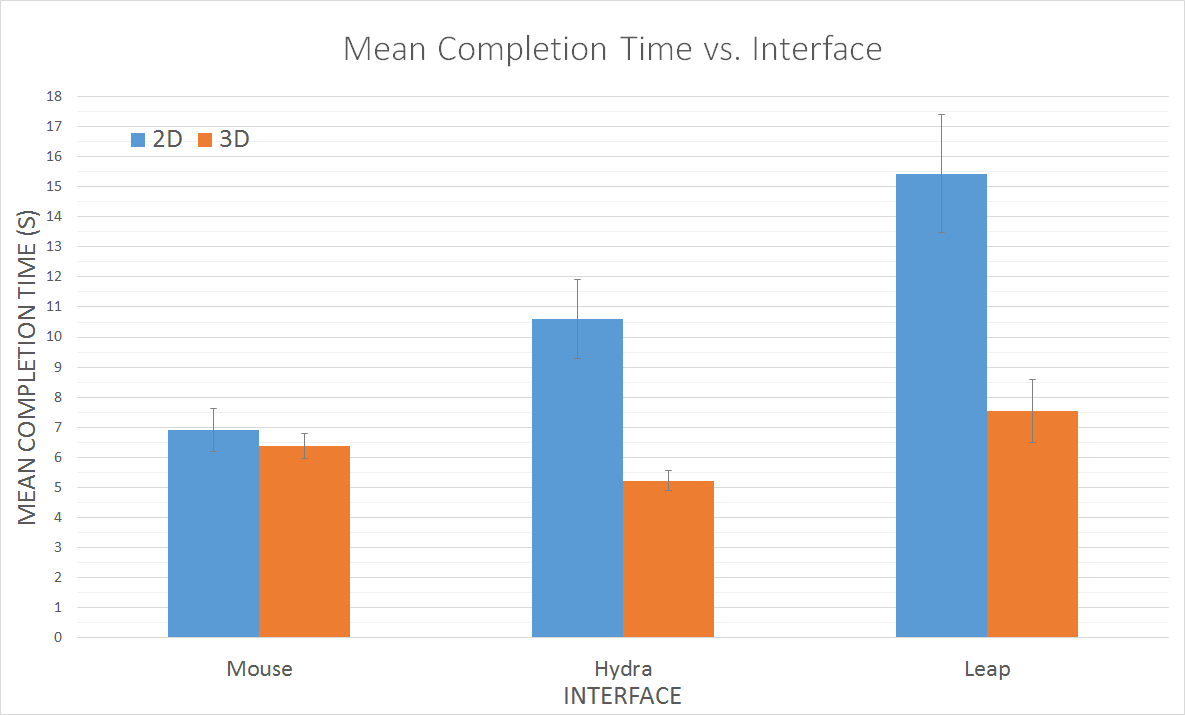
\includegraphics[width=\columnwidth]{timingmeans.png}
    \caption{Mean task completion times for each interface combination}
    \label{fig:means}
\end{figure}

The Repeated Measures ANOVA showed a strong main effect on task
completion time of Input ($F(1.25,11.2) = 8.94, p = 0.009$) and Output ($F(1,9)
= 36.8, p < 0.001$). This was qualified by an interaction between Input and
Output ($F(1.299,) = 11.6, p = 0.004$). \figref{fig:means} shows the means
of per-task completion times with 95\% confidence intervals.

From this data, we see that using the 3D stereoscopic output improved
completion times regardless of input interface used. The fastest input device in
the 2D output case was the mouse, while the Hydra resulted in the fastest mean
completion time overall when used with the 3D stereoscopic output (mean
completion time of $5.22$s).
We note that output interface did not improve performance with the mouse
($6.901$s vs. $6.370$s) as much as with the other two interfaces.

\begin{figure*}
    \centering
    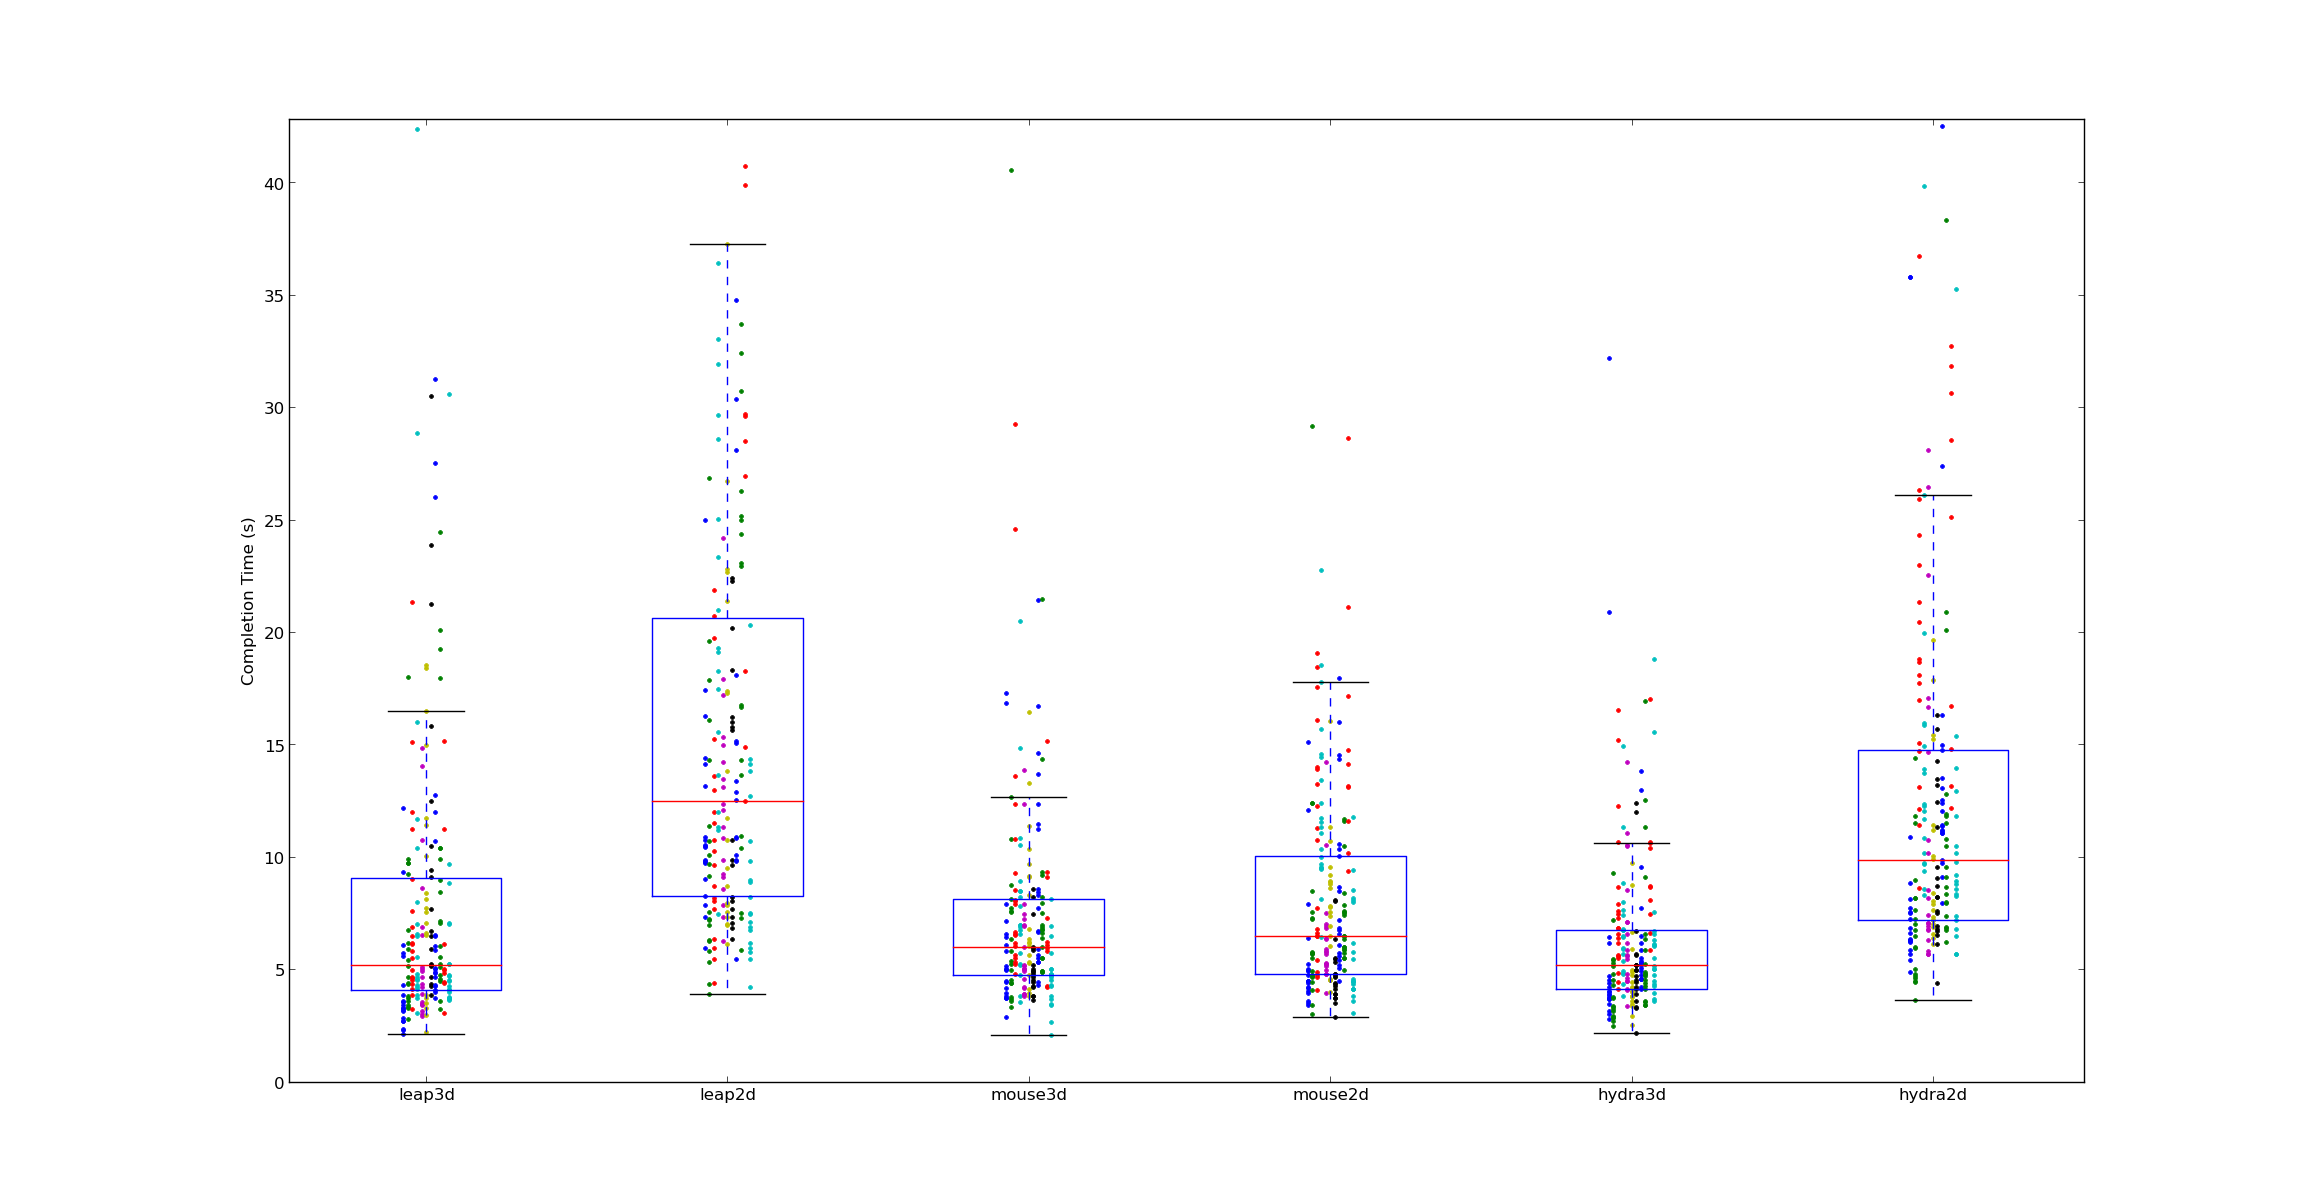
\includegraphics[width=\textwidth]{rawdata.png}
    \caption{Raw completion time data grouped by interface combination.
             Note that there are several outliers in the {\tt leap2d} that
             are outside the bounds of the plot.}
    \label{fig:rawtimes}
\end{figure*}

However, examining the raw data (\figref{fig:rawtimes}) shows that
the Leap had a particularly skewed distribution of completion times.
Using the median as a more robust measure of central tendency, we see
that using the Leap with the 3D output interface had comparable completion
times with the Hydra with 3D output, the fastest input device.

Observing participants during the experiment and reviewing post-experiment
surveys suggest that the Leap's long tail of high completion times occurs
primarily because of the Leap's tendency to lose track of the user's hands.
The Leap technology is still in development, so these results suggest that
performing this experiment with more robust in-air one-to-one input
system would yield more reliable results.
